


The Mueller matrix, or scattering matrix, describes the polarization properties of light scattered by the dust grains \citep{Kataoka_2015} and is calculated using \texttt{DSHARP}. Two relevant matrix elements are \Zoo and \ZootNS, which represent linear polarized scattering and total scattering, respectively \citep{Zhang2023}. The polarization fraction is given by the ratio $-Z_{12, \text{eff}}/Z_{11, \text{eff}}$ averaged over the grain size distribution \citep{Kataoka_2015}.  The polarization fraction depends on the scattering angle, as shown in Figure \ref{fig: Kataoka2015Figure2Recreation}. For smaller grain sizes, the polarization fraction peaks near a scattering angle of  90\deggNS. The polarization fraction from the model at  90\degg is denoted by $P$. 


% \begin{equation}
%     N_{11} = -\frac{Z_{12}}{Z_{11}}
%     \label{eq: N11}
% \end{equation}

Figure \ref{fig: Kataoka2015Figure2Recreation} shows the dependence of polarization fraction on scattering angle for different maximum grain sizes. For smaller dust grains (10 \micron and 100 \micronNS), the polarization fraction peaks near a scattering angle of 90\deggNS. For larger dust grains (1 mm and 1 cm), the polarization fraction remains much closer to zero, indicating that polarization from scattering is not efficient at larger grains. 



\begin{figure}[htbp]
  \centering
  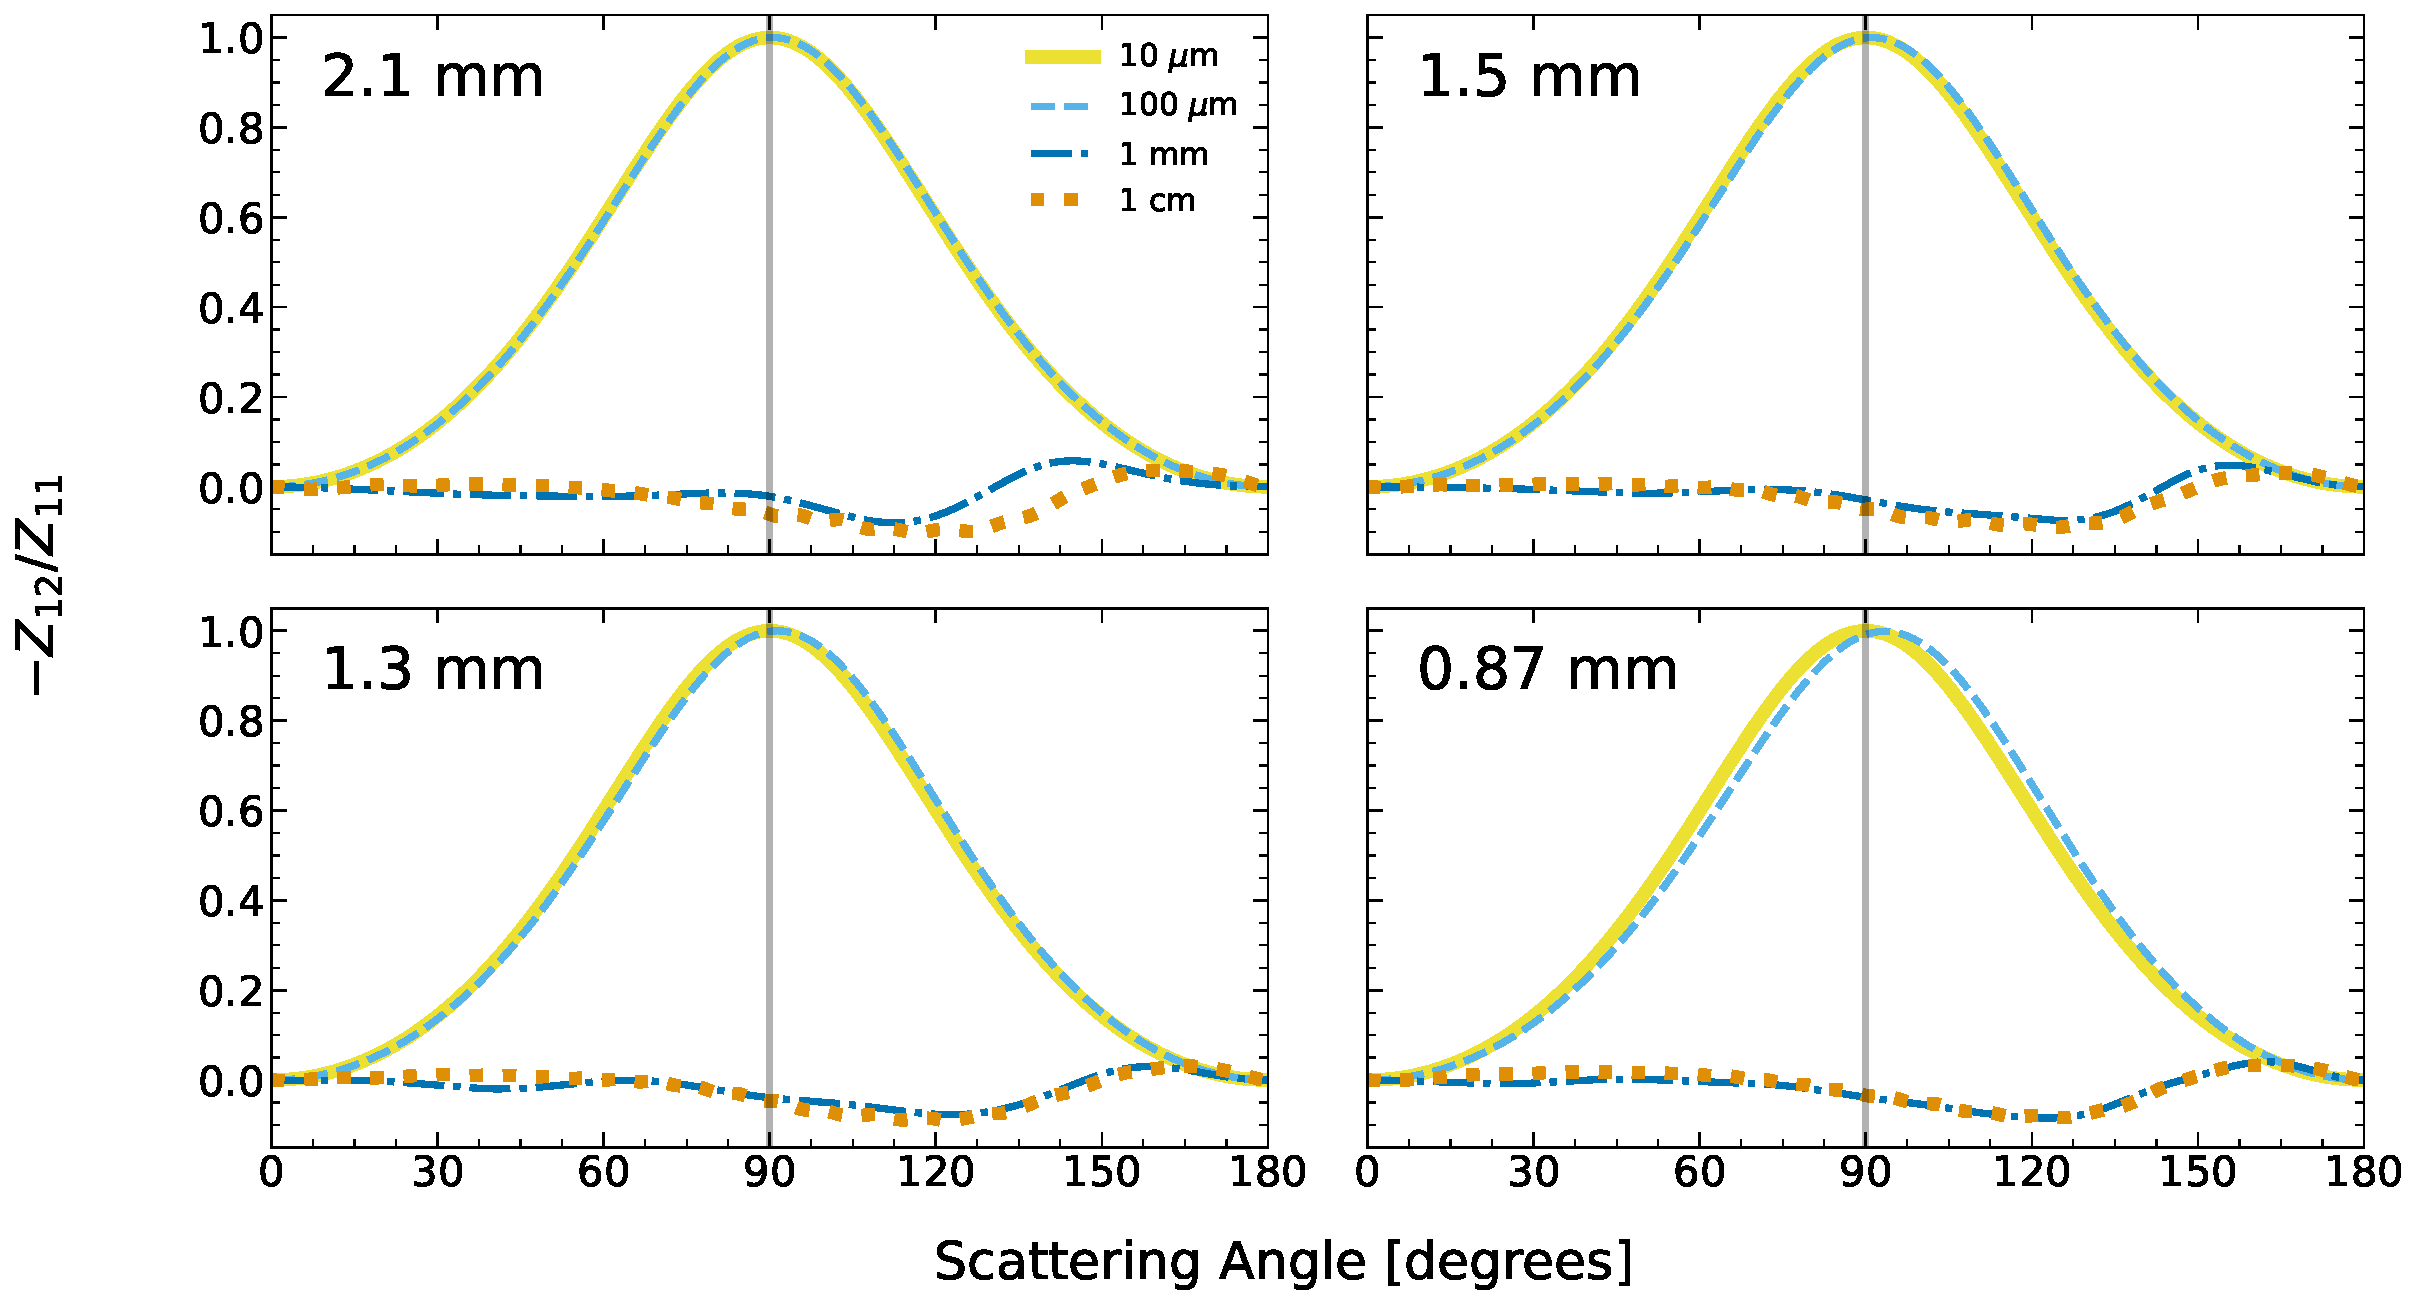
\includegraphics[width=0.99\textwidth]{WRITEUP_AND_IMAGES/IMAGES/WRITEUP/DustModels/Kataoka2015Fig2_grid.pdf}
  \caption{Polarization fraction as a function of scattering angle for maximum grain sizes of 10 \micronNS, 100 \micronNS, 1 mm and 1 cm for compact dust grains. This is a replication of Figure 2 from \cite{Kataoka_2015}. \coded{new colours} }
  \label{fig: Kataoka2015Figure2Recreation}
\end{figure}

% ----------------------------------------------




% ----------------------------------------------
% \subsubsection{Polarization and Albedo as a Function of Grain Size}
% \label{sec: c5_P_and_w_vs_a}

\note{Need to update this for both \weff and different porosities. Make sure there are references to Figure \ref{fig: Kataoka2015Figure3Recreation}, Figure \ref{fig: Pweff_vs_grainsize}, Table \ref{tab: amax_peak_values} and Figure \ref{fig: Pweff_vs_amax_porous}}


% ----------------------------------------------
Figure \ref{fig: Kataoka2015Figure3Recreation} shows the polarization fraction and effective albedo as a function of grain size. The polarization fraction is larger for smaller grains, and quickly drops off as the dust grains increase. Alternatively, the effective albedo increases with dust grain size, as there is more surface area for the light to reflect off of. The characteristic grain size for each wavelength is shown as a grey line (values listed in Table \ref{tab: amax_peak_values}). The characteristic grain size should approximately correlate to where the polarization and albedo curves are at their maximum, highlighting the wavelength dependence of polarization scattering. 


\begin{figure}[htbp]
  \centering
  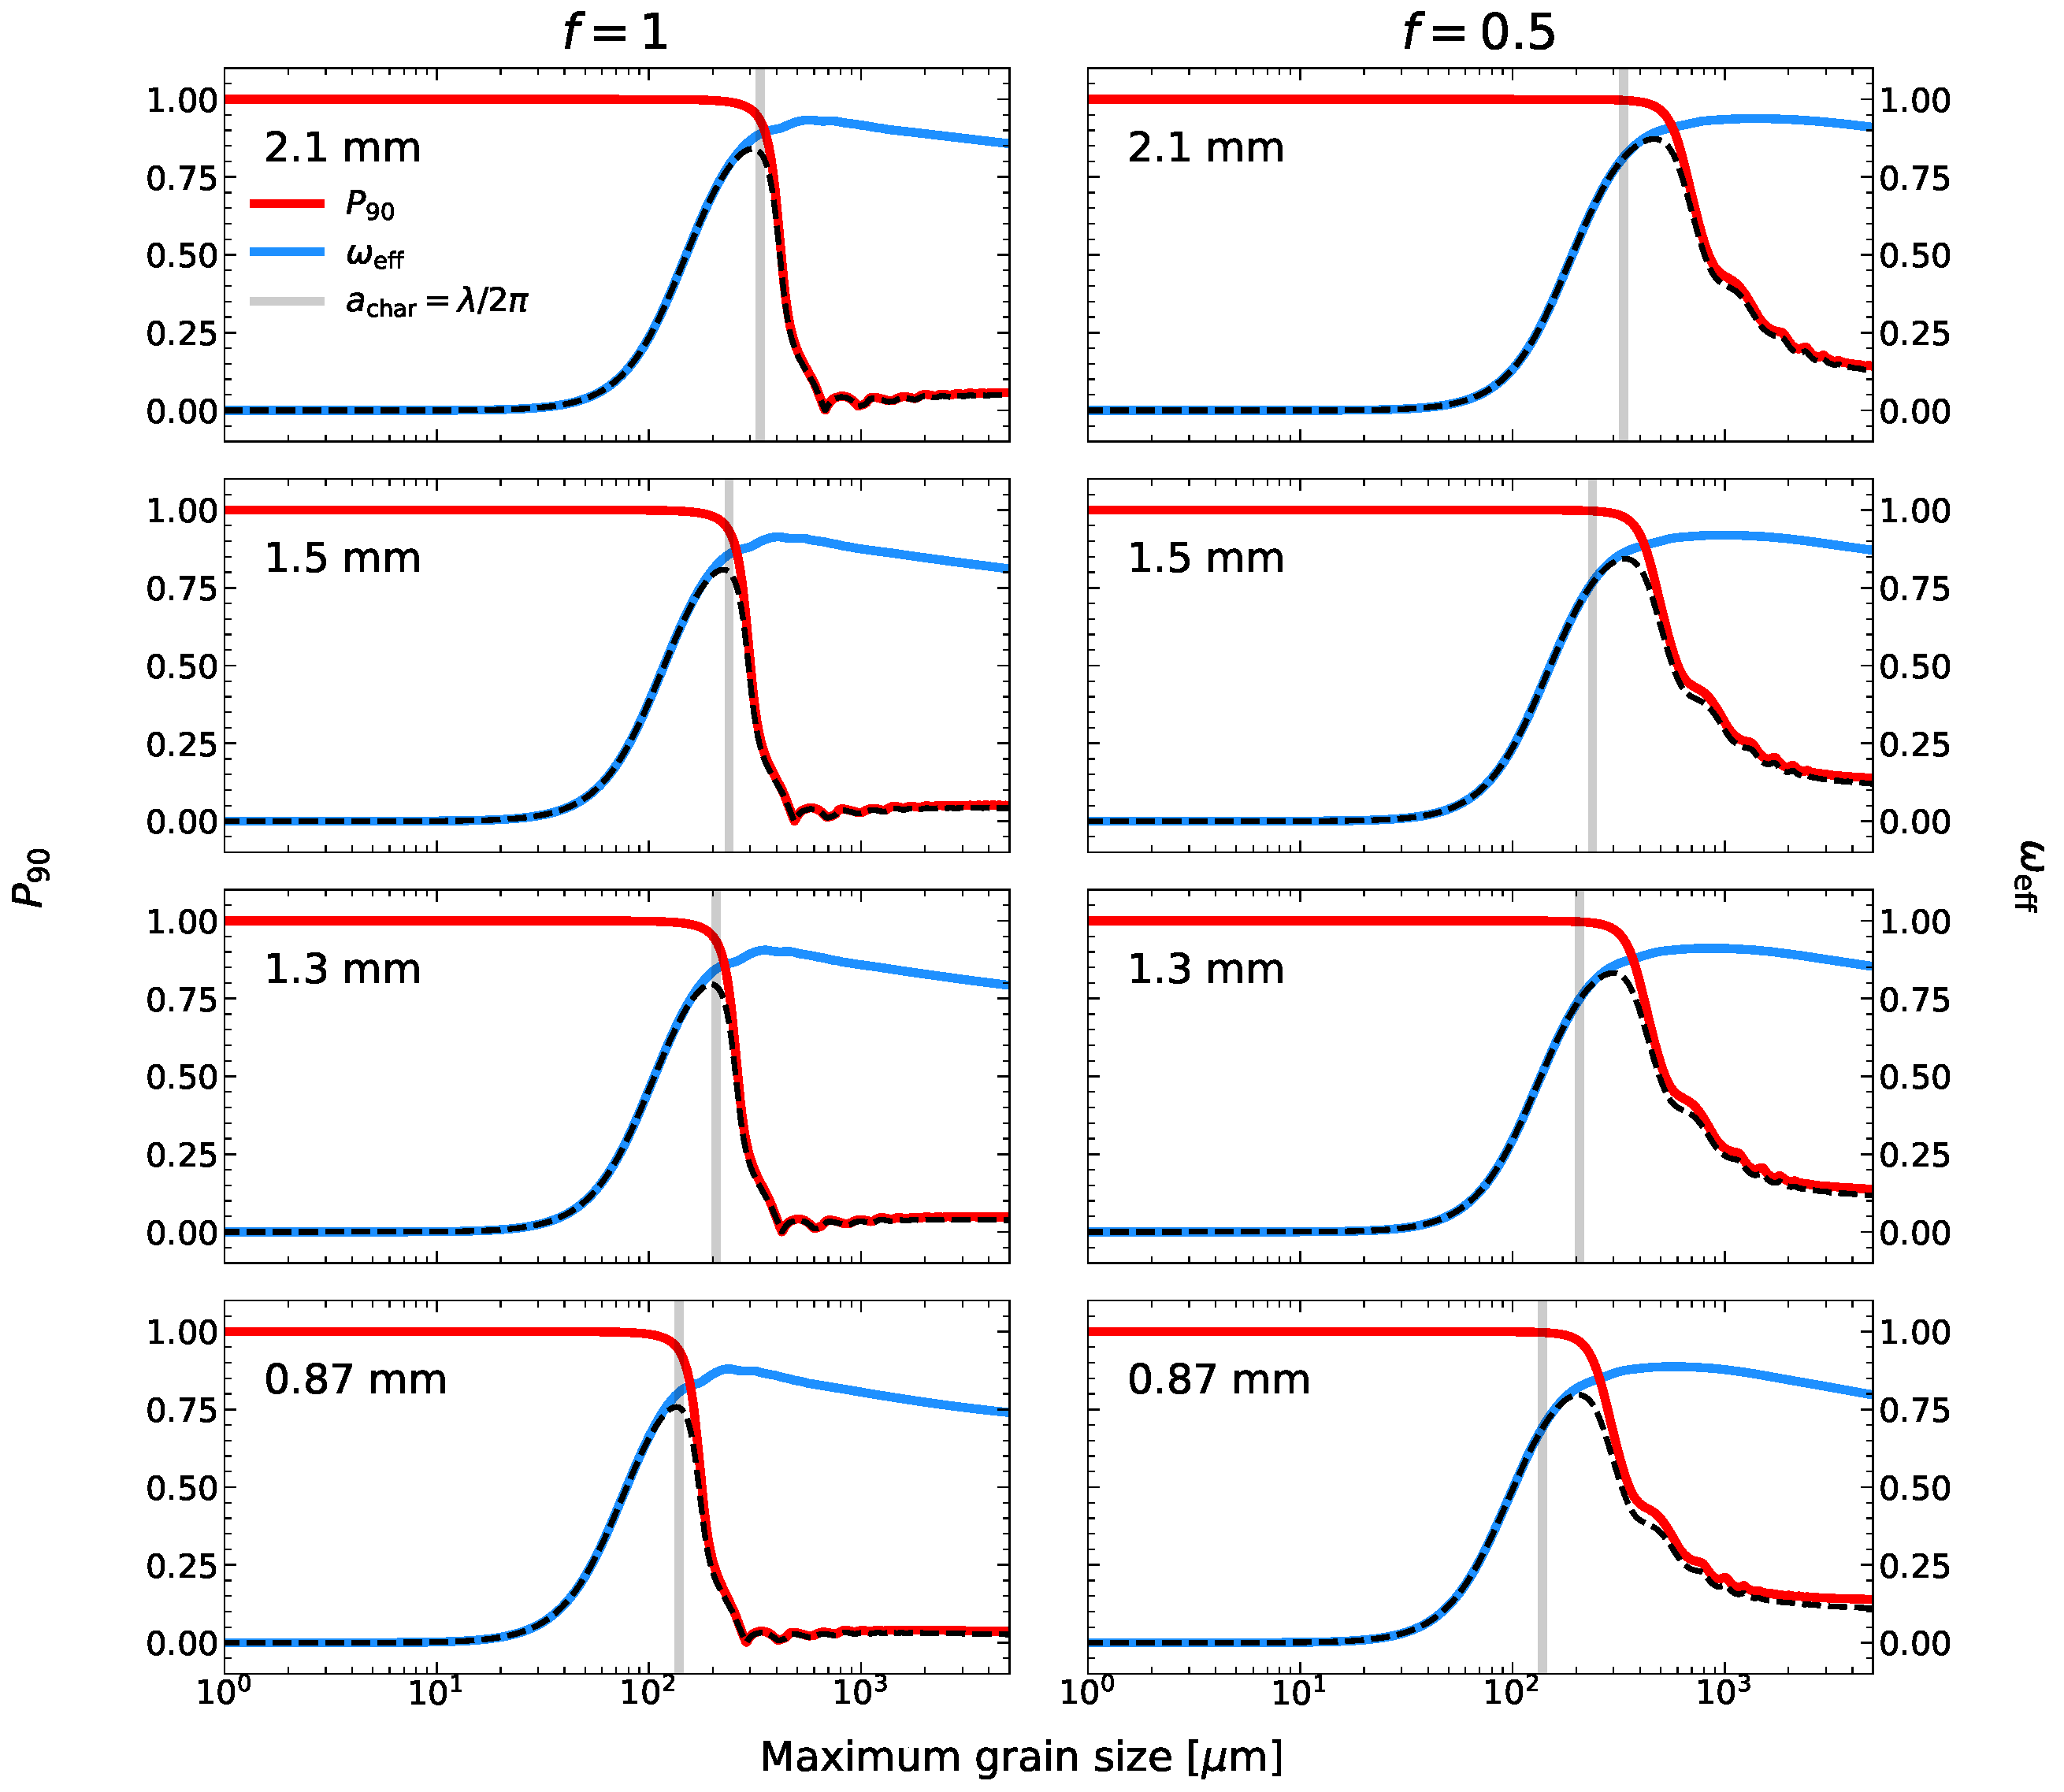
\includegraphics[width=0.99\textwidth]{WRITEUP_AND_IMAGES/IMAGES/WRITEUP/DustModels/P_vs_w_eff_vs_grainsize_grid_smooth_porosities.pdf}
  \caption{Plot of polarization fraction $P$ in red and effective albedo in blue as a function of grain size for compact dust grains. The characteristic grain size for each wavelength is overplotted in grey, highlighting that it roughly corresponds to the local maxima of both curves. This is a recreation of Figure 3 from \cite{Kataoka_2015}. }
  \label{fig: Kataoka2015Figure3Recreation}
\end{figure}

% ----------------------------------------------







% ----------------------------------------------

% ----------------------------------------------
% ----------------------------------------------


The product of the polarization fraction and the effective single-scattering albedo, \PweffNS, provides a measurement of the contribution of each grain size to the polarized scattered light at a specific observing wavelength. It can be used to determine the grain sizes that contribute the most to the observed polarization \citep{Kataoka_2015}. Figure \ref{fig: Pw_eff_vs_grainsize} shows the \Pweff curves for compact spherical and irregular grains as a function of maximum grain size, with the characteristic grain size plotted as well for comparison. 

compares the \Pweff curves and characteristic dust grain sizes for the observing wavelengths considered in this project assuming compact dust grains. The polarized scattering efficiency at each wavelength peaks at a grain size close to the characteristic grain size, shown plotted with a dashed line in the respective colour. The peaks occur at grain sizes of approximately hundreds of microns, indicating that polarization observations at these wavelengths are most sensitive to grains in this range. As discussed in Chapter \ref{sec: intro_mw}, using multi-wavelength observations allows the different wavelengths to be fit simultaneously, providing a better constraint on the grain size. How this is done is explained in Chapter \ref{sec: ch5_determining_abest}. 





% % ----------------------------------------------
% \subsubsection{P$\boldsymbol{\omega}$ as a Function of Grain Size \note{bold}}
% \label{sec: c5_P_and_a}
% % ----------------------------------------------






% ------------------------------------------------------
\begin{table}[h!]
\centering
\caption{Maximum grain size corresponding to the peak \Pweff value for compact grains, and characteristic grain size as a dashed line for each wavelength in Figure \ref{fig: Pw_eff_vs_grainsize}. }
\label{tab: amax_peak_values}
\begin{tabular}{lcccc}
\toprule
\textbf{Grain Size ($\boldsymbol{\mu}$m)} & \textbf{\bfour} & \textbf{\bfive} & \textbf{\bsix} & \textbf{\bseven} \\
\midrule

$a_{\text{char}}$
& 334.23
& 238.73
& 206.90
& 138.46 \\

$a_{\max}$ (spherical, compact)
& 307.88
& 223.71
& 196.46
& 134.50 \\


$a_{\max}$ (spherical, porous)
& 464.55
& 339.38
& 298.04
& 204.05 \\


$a_{\max}$ (irregular)
& 330.59
& 238.90
& 211.60
& 145.32 \\



\bottomrule
\end{tabular}
\label{tab: amax_peak_values}
\end{table}
% ------------------------------------------------------





% ----------------------------------------------
\begin{figure}[htbp]
  \centering

  \begin{minipage}[t]{0.48\textwidth}
    \centering
    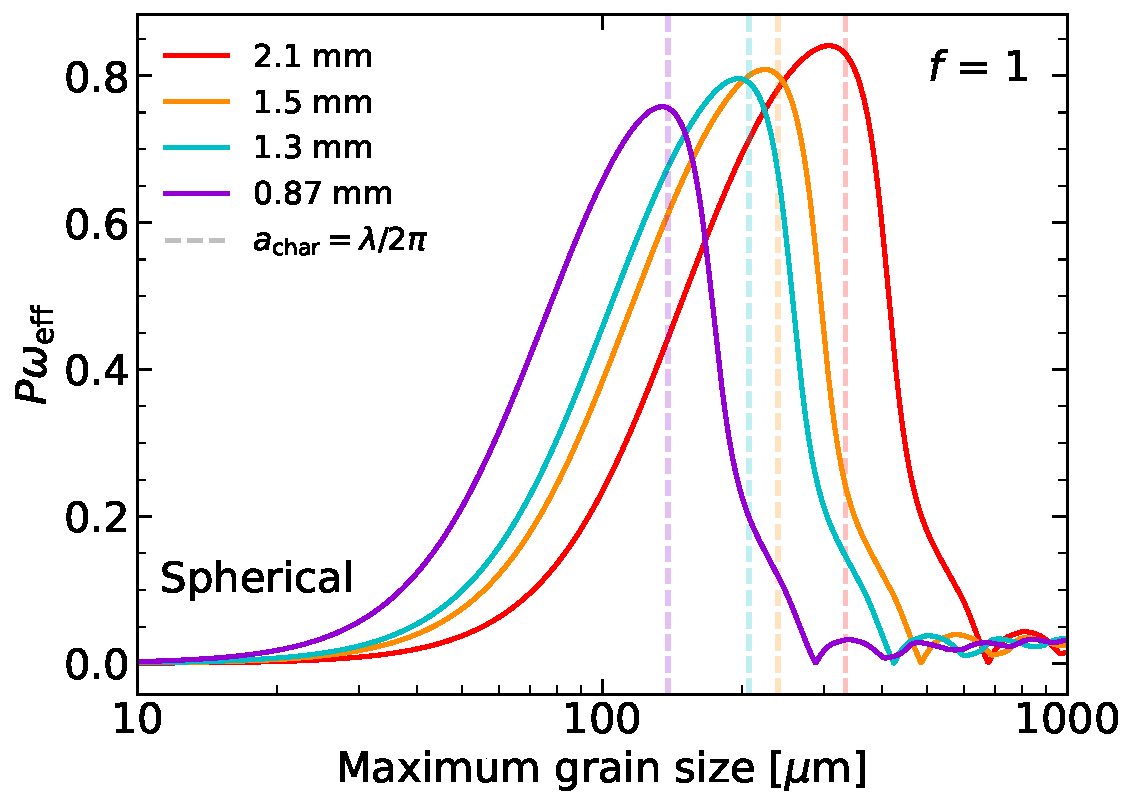
\includegraphics[width=\textwidth]{WRITEUP_AND_IMAGES/IMAGES/WRITEUP/DustModels/Pw_eff_vs_grainsize_compact.pdf}
  \end{minipage}
  \hfill
  \begin{minipage}[t]{0.48\textwidth}
    \centering
    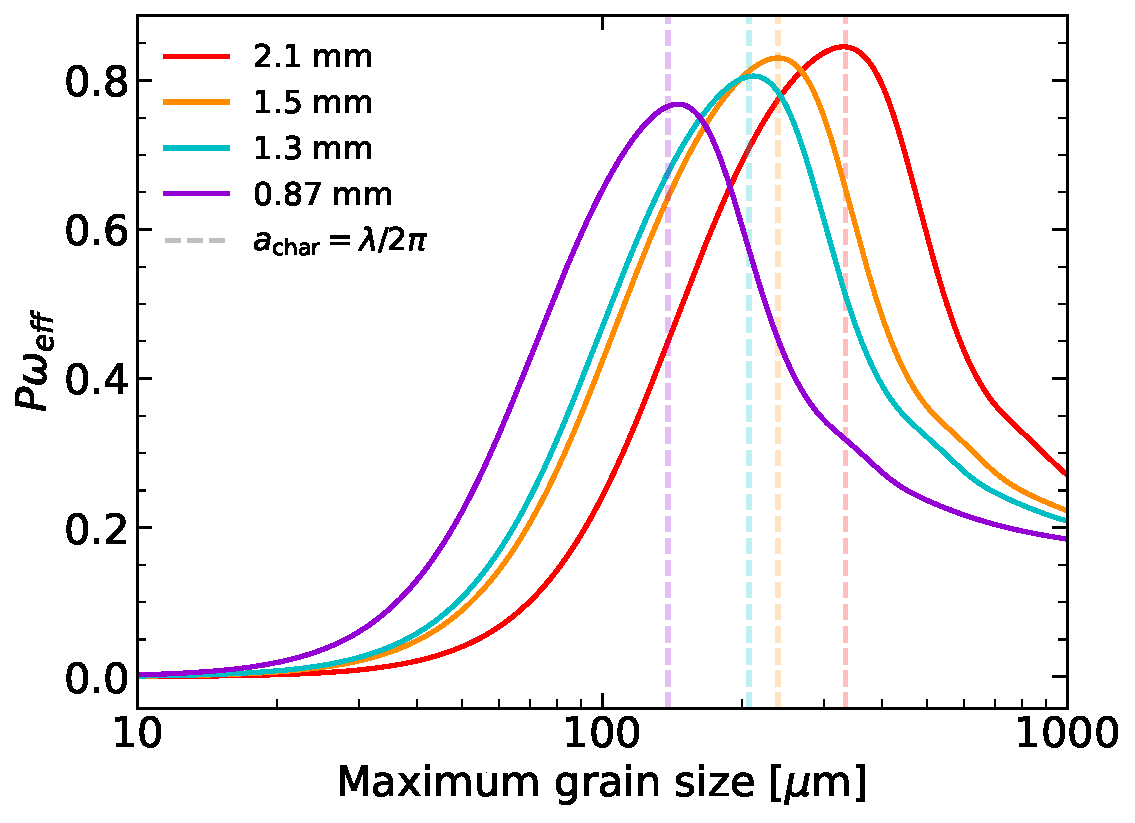
\includegraphics[width=\textwidth]{WRITEUP_AND_IMAGES/IMAGES/WRITEUP/glitterin/Pw_eff_vs_grainsize.pdf}
  \end{minipage}
  \caption{Polarization curves (\PweffNS) versus grain size for each wavelength for spherical grains (left) and irregular grains (right), for compact dust grains. Overplotted as a dashed line with matching colour is the characteristic grain size. Locations of maximum \Pweff and characteristic grain size are listed in Table \ref{tab: amax_peak_values}.  \coded{*Added spherical label, *Added irregular label}}
  \label{fig: Pweff_vs_grainsize}
\end{figure}
% ----------------------------------------------







% \noindent \question{Should I add any replications of \cite{Zhang2023} plots? Should I add a section about replicating plots from glitterin? This could be replicating these plots from Kataoka with glitterin, or replicating the plots Daniel presented in his paper}



% \noindent \SC{A: I think if you add a few cases of porous grains and indicate that these are consistent with Zhang et al., that is fine.  You could give the final P*omega plot for glitterin.  I don't think you need to show examples of opacity, polarization fraction, etc. for all cases.  These are illustrations to show what you are calculating.  The methodology is similar.  What changes are the dust properties that affect opacity and the refractive indices.}

% ----------------------------------------------
%
%
%
%
%

%

